\documentclass[dvipsnames]{beamer}

\mode<presentation> {
    \usetheme{Szeged}
    \usecolortheme{beaver}
}

% \usepackage{subfig}

% Tables
\usepackage{tabularx}

% Graphics
\usepackage{xcolor}
\usepackage{graphicx}
\graphicspath{{Figures/}}

% Math
\usepackage{amssymb}
\usepackage{mathtools}
\usepackage{bm}
\usepackage{fancyvrb} % for "\Verb" macro
% Relations between variables
\DeclareMathOperator*{\CI}{{\,\perp\mkern-12mu\perp\,}}
\DeclareMathOperator*{\nCI}{{\,\not\mkern-1mu\perp\mkern-12mu\perp\,}}
\DeclareMathOperator*{\SEP}{\perp}
\DeclareMathOperator*{\nSEP}{\not\perp}
\newcommand{\indep}[4]{{#1} \CI_{#4} {#2} \given {#3}}
\newcommand\dep[4]{{#1} \nCI_{#4} {#2} \given {#3}}
\newcommand\sep[4]{{#1} \SEP_{#4} {#2} \given {#3}}
\newcommand\con[4]{{#1} \nSEP_{#4} {#2} \given {#3}}
\newcommand{\dsep}[4]{{#1} \SEP_{#4}^d {#2} \given {#3}}
\newcommand{\dcon}[4]{{#1} \nSEP_{#4}^d {#2} \given {#3}}
\newcommand{\sigmasep}[4]{{#1} \SEP_{#4}^\sigma {#2} \given {#3}}
\newcommand{\sigmacon}[4]{{#1} \nSEP_{#4}^\sigma {#2} \given {#3}}
\newcommand{\Prb}{\mathbb{P}}
\newcommand{\marg}[1]{\mathrm{marg}_{#1}}
\newcommand{\intervene}{\mathrm{do}}
% Bold, cursive
\newcommand\B[1]{\bm{#1}}
\newcommand\C[1]{\mathcal{#1}}
\newcommand\BC[1]{\bm{\mathcal{#1}}}
% Arrows (oriented, star, circle)
\newcommand{\ot}{\leftarrow}
\newcommand{\oto}{\leftrightarrow}
\newcommand{\ots}{\leftarrow\mkern-13mu\ast\,}
\newcommand{\otc}{\leftarrow\mkern-9mu\circ\,}
\newcommand{\sto}{\,\ast\mkern-13mu\to}
\newcommand{\stt}{\,\ast\mkern-13mu\relbar\!\!\!\relbar}
\newcommand{\tts}{\relbar\!\!\!\relbar\mkern-13mu\ast\,}
\newcommand{\sts}{\,\ast\mkern-10mu\relbar\mkern-10mu\ast\,}
\newcommand{\ctc}{\,\circ\mkern-9mu\relbar\mkern-9mu\circ\,}
\newcommand{\cto}{\,\circ\mkern-9mu\rightarrow}
% Graph relations
\newcommand\mathbfsc[1]{\text{\normalfont\scshape#1}}
\newcommand\Det[1]{\mathbfsc{Det}(#1)}
\newcommand\an[1]{\mathbfsc{an}(#1)}
\newcommand\de[1]{\mathbfsc{de}(#1)}
\newcommand\scc[1]{\mathbfsc{sc}(#1)}
\newcommand\pa[1]{\mathbfsc{pa}(#1)}
\newcommand\ch[1]{\mathbfsc{ch}(#1)}
\newcommand\ncol[1]{\mathbfsc{ncol}(#1)}
\newcommand\col[1]{\mathbfsc{col}(#1)}
\newcommand\Detsub[2]{\mathbfsc{Det}_{#2}(#1)}
\newcommand\ansub[2]{\mathbfsc{an}_{#1}(#2)}
\newcommand\desub[2]{\mathbfsc{de}_{#1}(#2)}
\newcommand\sccsub[2]{\mathbfsc{sc}_{#1}(#2)}
\newcommand\pasub[2]{\mathbfsc{pa}_{#1}(#2)}
\newcommand\chsub[2]{\mathbfsc{ch}_{#1}(#2)}
% Names
\newcommand\mec{\mathbfsc{mec}}
% Other
\newcommand\given{\,|\,}

% Commands for presentation
\newcommand{\twoimg}[2]{
    \begin{columns}
        \begin{column}{0.5\textwidth}
            \includegraphics[width=\textwidth]{#1}
        \end{column}
        \begin{column}{0.5\textwidth}
            \includegraphics[width=\textwidth]{#2}
        \end{column}
    \end{columns}
}


\begin{document}

\title[Order-Based Causal Analysis]{Order-Based Causal Analysis \\ of Gene Expression Data} % The short title appears at the bottom of every slide, the full title is only on the title page

\author{Silvan de Boer} % Your name
\institute[UvA] % Your institution as it will appear on the bottom of every slide, may be shorthand to save space
{
University of Amsterdam \\ \medskip
\textit{silvandeboer@gmail.com} % Your email address
}
\date{\today} % Date, can be changed to a custom date



\begin{frame}
    \titlepage 
\end{frame}

\AtBeginSection[]{
    \begin{frame}
        \frametitle{Table of Contents}
        \tableofcontents[currentsection]
    \end{frame}
}

\begin{frame}
    \frametitle{Table of Contents}
    \tableofcontents
\end{frame}

% \section{Introduction}

% Causality: statistical + symbolic AI
\begin{frame}
    \frametitle{Artificial Intelligence}
    \begin{itemize}
        \item Statistical Artificial Intelligence
            \begin{itemize}
                \item Deduction
                \item Data
                \item Opaque
            \end{itemize}
        \item Symbolic Artificial Intelligence
            \begin{itemize}
                \item Induction
                \item Knowledge
                \item Interpretable
            \end{itemize}
    \end{itemize}
\end{frame}

\begin{frame}
    \frametitle{Statistical Artificial Intelligence}
    
    \only<1>{
        \twoimg{1introduction/stat1.png}{1introduction/stat1appl.jpg}
    }
    \only<2>{
        \twoimg{1introduction/stat2.png}{1introduction/stat2appl.jpeg}
    }
    \only<3>{
        \twoimg{1introduction/stat3.jpeg}{1introduction/stat3appl.png}
    }
\end{frame}

\begin{frame}
    \frametitle{Symbolic AI}
    
    \only<1>{
        \twoimg{1introduction/symb1}{1introduction/symb1appl}
    }
    \only<2>{
        \twoimg{1introduction/symb2}{1introduction/symb2appl}
    }
    \only<3>{
        \twoimg{1introduction/symb3}{1introduction/symb3appl}
    }
\end{frame}

% Questions answerable with causality (encoding causal assumptions)
\begin{frame}
    \frametitle{Causality}

    \only<1>{
        \twoimg{1introduction/joint_distr}{1introduction/rct}
    }

    \only<2-3>{
        \begin{columns}
            \begin{column}{0.4\textwidth}
                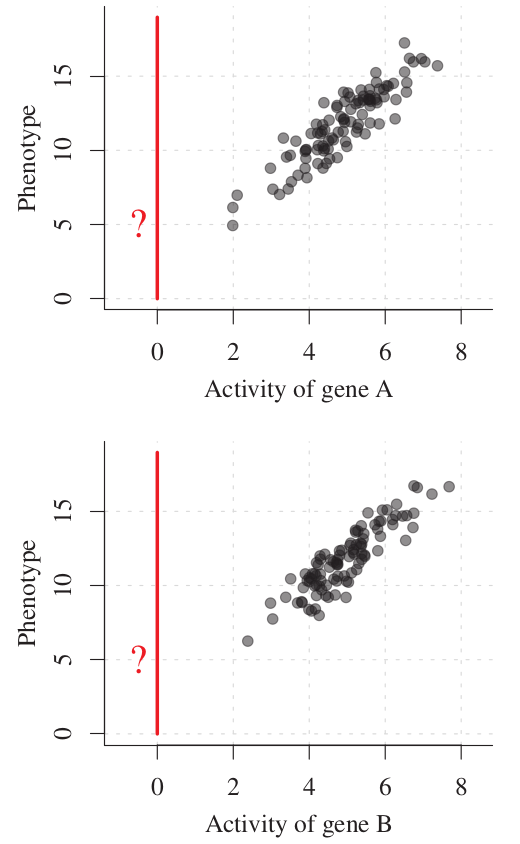
\includegraphics[width=\textwidth]{1introduction/causalknowledgeA.png}
            \end{column}
            \begin{column}{0.4\textwidth}
                \includegraphics<3>[width=\textwidth]{1introduction/causalknowledgeB.png}
            \end{column}
        \end{columns}
    }

    % Questions answerable by causality
    
    
    
\end{frame}




% Modeling causality: SCMs to encode causal assumptions (focus?: math or methods)


\begin{frame}
    \frametitle{Structural Causal Model}
    
\end{frame}


% Inspiration: Philips LCD (+ state-of-the-art)


% Aims and challenges




% \section{Data Understanding}

\begin{frame}
    \frametitle{Data Understanding}

    First slide

\end{frame}

\begin{frame}
    \frametitle{Data Understanding}

    Second slide

\end{frame}

\section{Algorithm Design}

\begin{frame}
    \frametitle{Introduction}

    First slide

\end{frame}

\begin{frame}
    \frametitle{Introduction}

    Second slide

\end{frame}

% \section{Analysis}

\begin{frame}
    \frametitle{Experiments}

    \only<1>{
        Set-up
        \begin{itemize}
            \item 5 data folds
            \item 100 $\times$ 50\% subsamples
            \item L$_2$-boosting preselection
        \end{itemize}
    }

    \only<2>{
        Methods
        \begin{itemize}
            \item Baselines: random, L$_2$-boosting
            \item Comparison: LCD, boosted LCD, ICP
            \item Ablations: random order and/or positions
        \end{itemize}
    }

    \only<3>{
        Evaluation
        \begin{itemize}
            \item Prediction method: discrete, continuous
            \item Ground-truth for ROC: 3 thresholds, absolute and standardized
            \item Norm for regression deviation: $l_1$-norm, $l_2$-norm
            \item Data: all, intervention table, order-compliant relations
        \end{itemize}
    }
\end{frame}



\begin{frame}
    \frametitle{Similarity to LCD}

    \only<1>{
        \begin{center}
            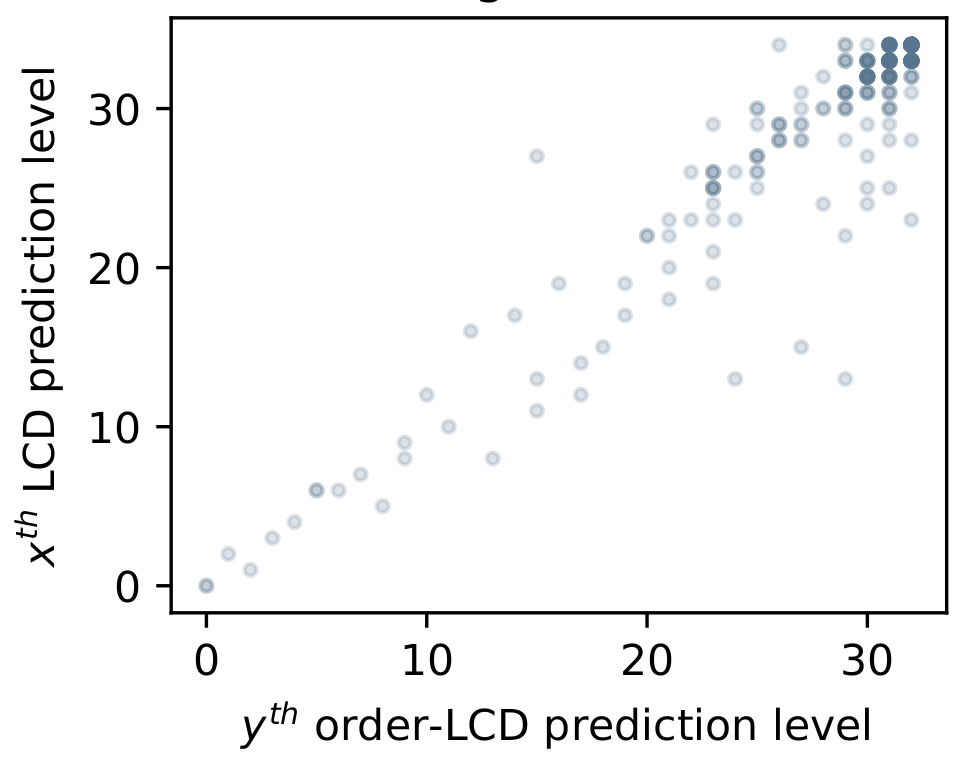
\includegraphics[height=.8\textheight]{4analysis/olcd_vs_lcd.png}
        \end{center}
    }

    \only<2>{
        \begin{center}
            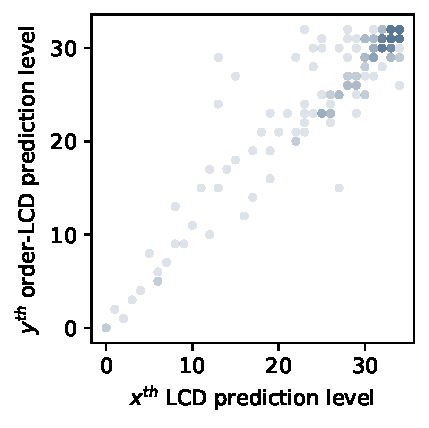
\includegraphics[width=\textwidth]{paper/7score_vs}
        \end{center}
    }

    \only<3>{
        \begin{center}
            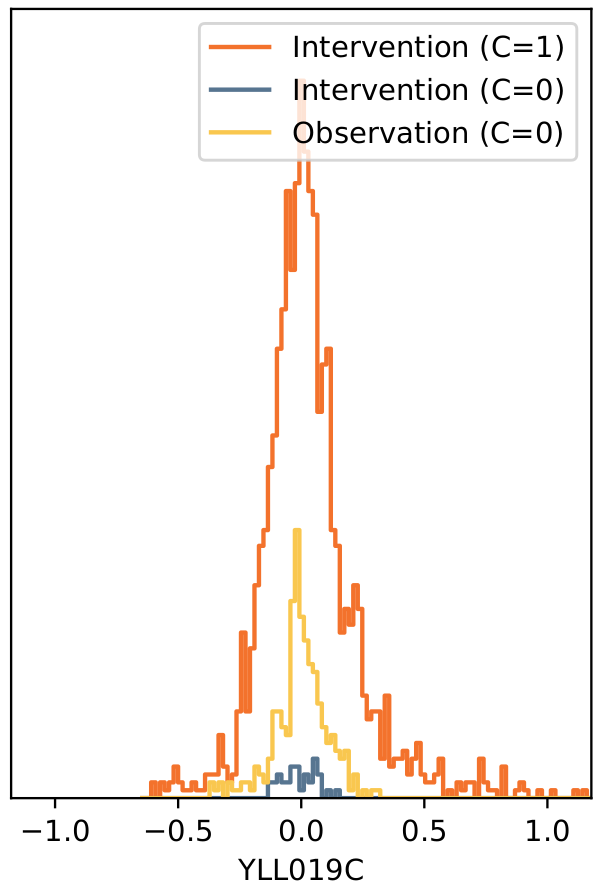
\includegraphics[height=.8\textheight]{4analysis/context_hist_strongest.png}
        \end{center}
    }

    \only<4>{
        \begin{center}
            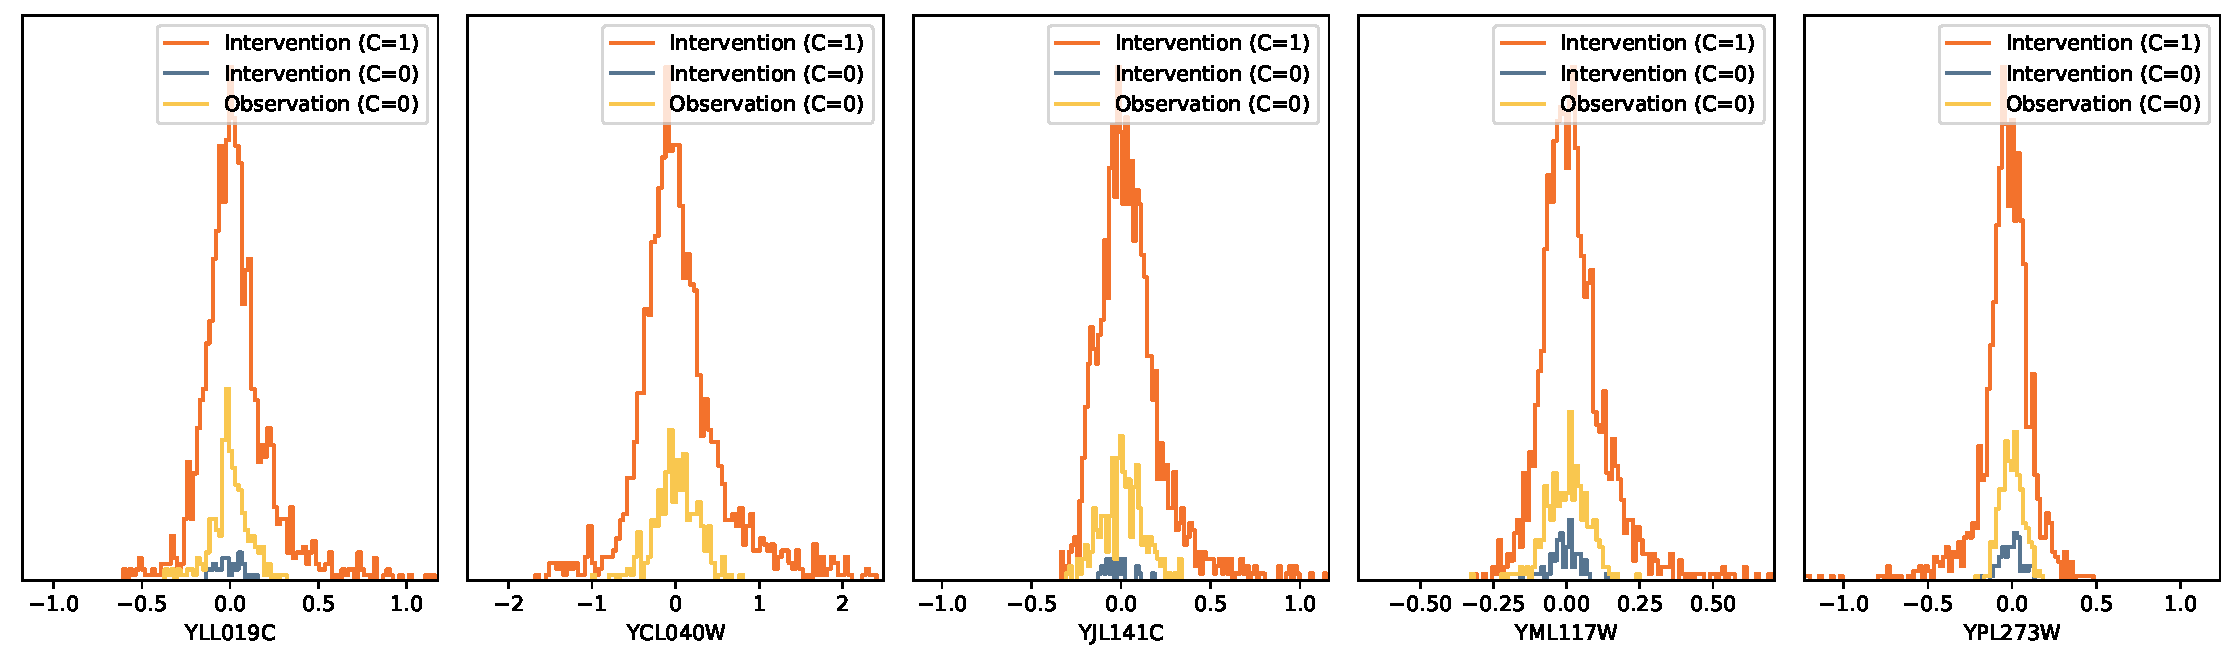
\includegraphics[width=\textwidth]{paper/7context_hist}
        \end{center}
    }

\end{frame}

\begin{frame}
    \frametitle{Quantitative Results}


    \only<1>{
        \begin{center}
            \includegraphics[width=\textwidth]{4analysis/roc_method}
        \end{center}
    }

    \only<2>{
        \begin{center}
            \includegraphics[width=\textwidth]{4analysis/roc_lcd}
        \end{center}
    }

    \only<3>{
        \begin{center}
            \includegraphics[height=.8\textheight]{4analysis/regression_example}
        \end{center}
    }

    \only<4>{
        \begin{center}
            \includegraphics[width=\textwidth]{4analysis/cont_method}
        \end{center}
    }

    \only<5>{
        \begin{center}
            \includegraphics[width=\textwidth]{4analysis/cont_lcd}
        \end{center}
    }
    

\end{frame}

% \section{Outlook}

% Contributions
\begin{frame}
    \frametitle{Contributions}

    \only<1>{
        \begin{itemize}
            \item Properties of the data set
            \item Penalty ratio metric
            \item Thorough analysis of order methods
            \item Design of order-based LCD
            \item New quantitative and qualitative evaluation approaches
        \end{itemize}
    }

\end{frame}



\begin{frame}
    \frametitle{Outlook}

    % Theoretical questions
    \only<1>{
        Theoretical questions
        \begin{itemize}
            \item Order and positions are inferred from the data
            \item How valid is the exogeneity assumption?
            \item What functional relations between data and context are allowed?
            \item What implicit assumptions are required for the current method?
        \end{itemize}
    }

    % Further testing: simulation, different data
    \only<2>{
        Further testing
        \begin{itemize}
            \item Simulation
            \item Different data sets
        \end{itemize}
    }

    % Method adaptation: gradual and radical
    \only<3>{
        Adaptations to the method
        \begin{itemize}
            \item Gradual
                \begin{itemize}
                    \item More spread-out position estimates
                \end{itemize}
            \item Radical
                \begin{itemize}
                    \item Using continuous data
                    \item Joint estimate of order and position
                    \item Partial order
                    \item More use of known intervention targets
                \end{itemize}
        \end{itemize}
    }

    % Back to statistical and symbolic synergy: symbolic AI is hard
    \only<4>{
        \frametitle{One Step Closer to Human-Level Machine-Intelligence?}

        \begin{center}
            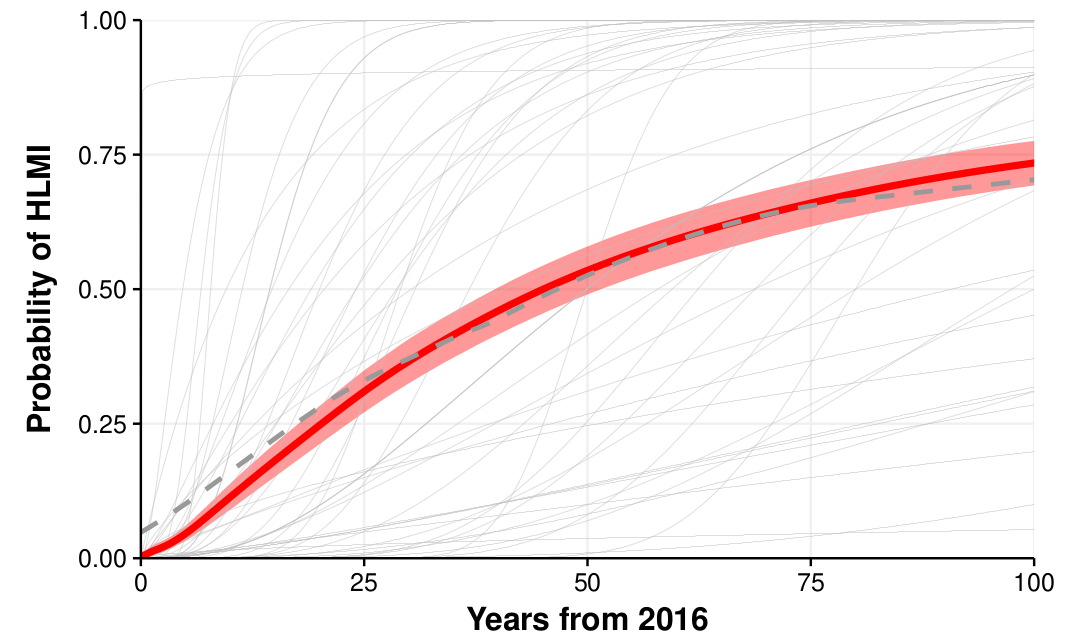
\includegraphics[width=.8\textwidth]{1introduction/hlmi.png}
        \end{center}

    }
    

\end{frame}

% \section*{Extra}

\begin{frame}
    % Back to statistical and symbolic synergy: symbolic AI is hard
    \only<1>{
        \frametitle{Top Order-Based LCD Predictions}
        \begin{center}
            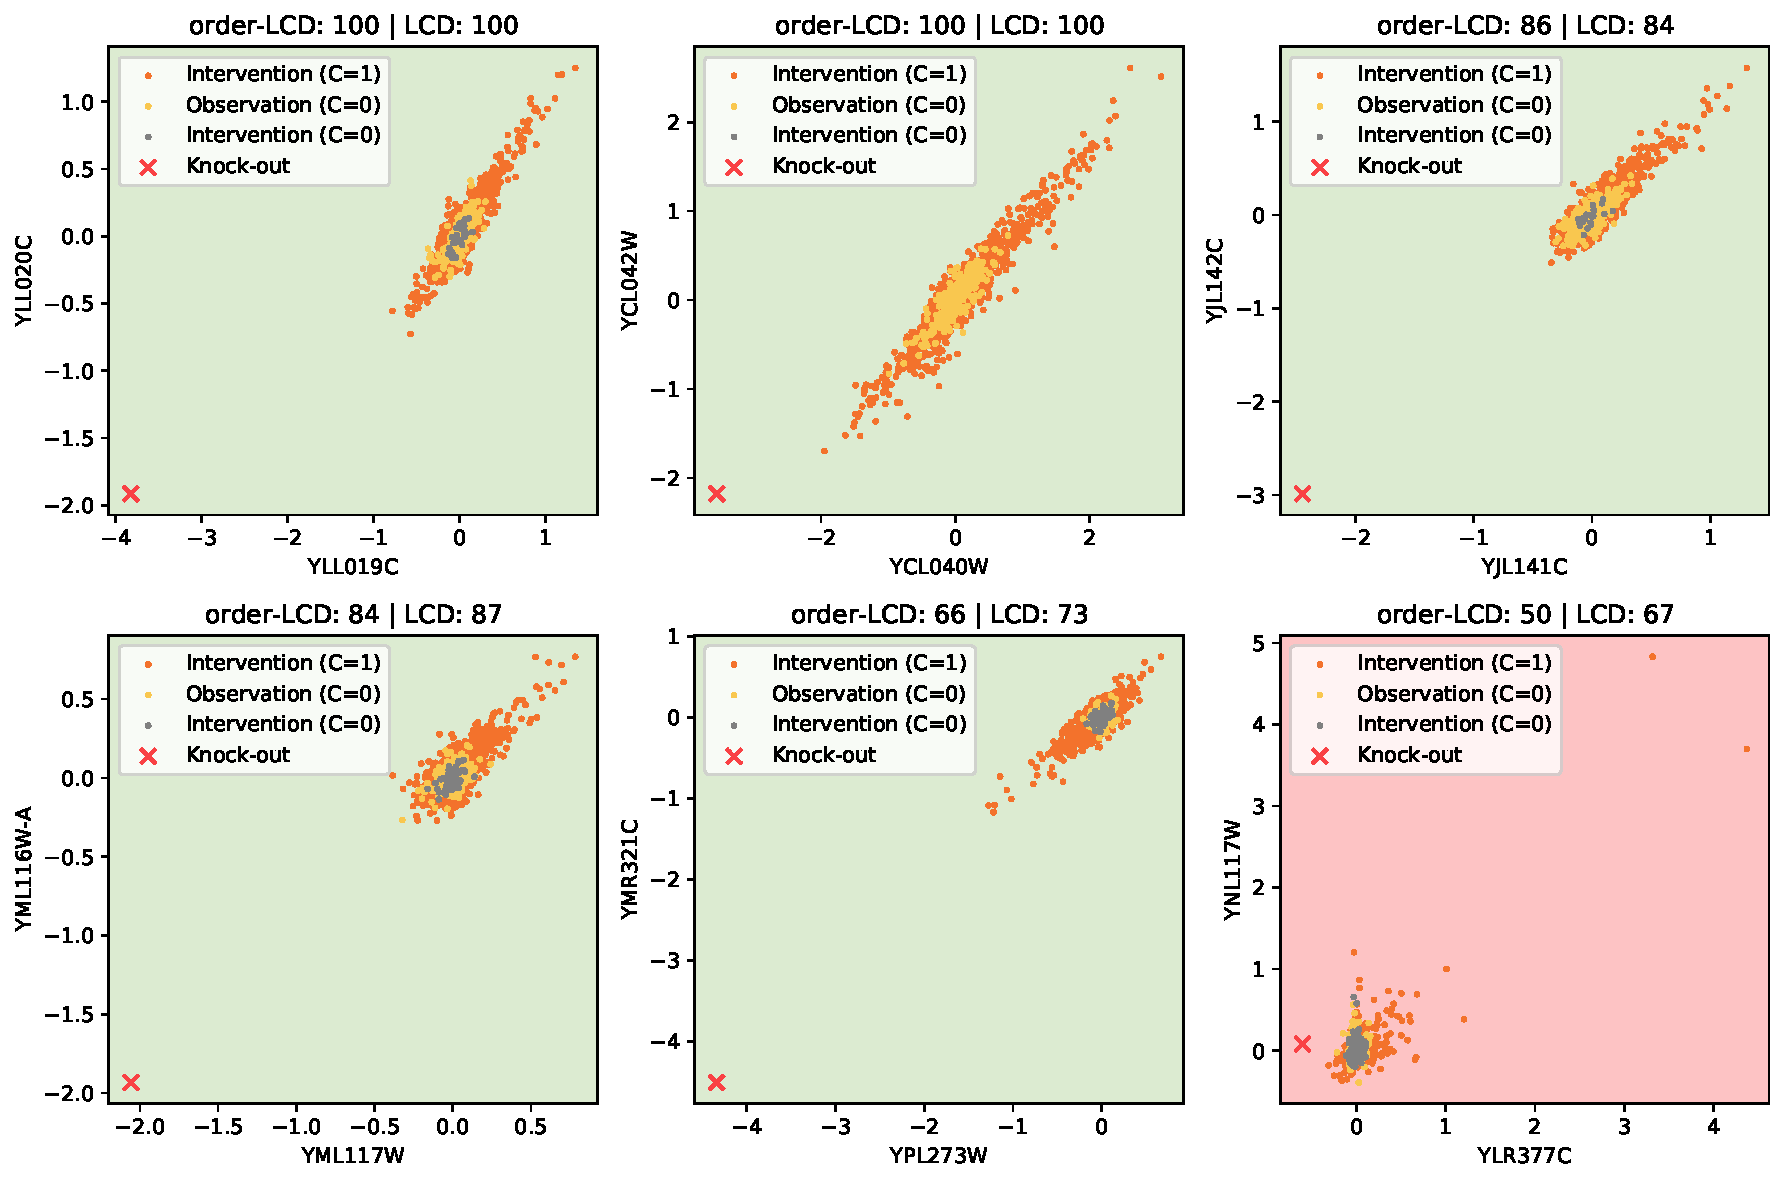
\includegraphics[width=.8\textwidth]{paper/7inclusive}
        \end{center}
    }

    \only<2>{
        \frametitle{TrueSkill Factor Graph}
        \begin{center}
            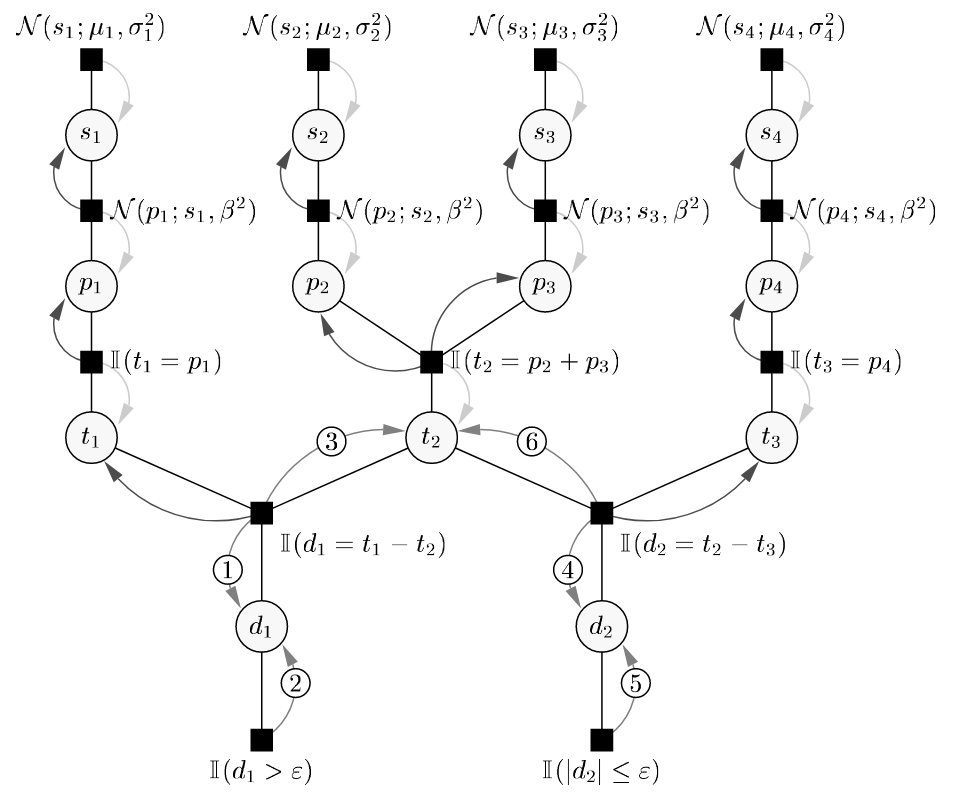
\includegraphics[width=.6\textwidth]{5extra/trueskill_factor_graph.png}
        \end{center}
    }
    

\end{frame}

\end{document}